\documentclass[conference]{IEEEtran}
\usepackage[T1]{fontenc}
\usepackage{graphicx}
\usepackage{booktabs}
\usepackage{array}
\usepackage{amsmath}
\usepackage{url}
\usepackage[hidelinks]{hyperref}

% Every measured number below comes from generated/numbers.tex, written by
% `python scripts/reproduce.py --from-results results`. Do not type results by hand.
% Generated by scripts/reproduce.py. Do not edit by hand.
\newcommand{\ErmMean}{7.87}
\newcommand{\ErmSD}{0.77}
\newcommand{\MixMean}{11.48}
\newcommand{\MixSD}{5.62}
\newcommand{\DiffMean}{-3.61}
\newcommand{\DiffSD}{5.62}
\newcommand{\MixWins}{1}
\newcommand{\PaperErm}{5.6}
\newcommand{\PaperMix}{4.2}
\newcommand{\PaperGain}{1.4}
\newcommand{\GapToPaperErm}{2.27}
\newcommand{\GapToPaperMix}{7.28}
\newcommand{\EpochSeconds}{60}
\newcommand{\GpuHours}{5.0}
\newcommand{\PeakGpuMB}{854}
\newcommand{\SourceHash}{dfcc812ed13b}
\newcommand{\ErmCleanTrain}{0.46}
\newcommand{\MixCleanTrain}{15.72}
\newcommand{\ErmValBN}{7.14}
\newcommand{\MixValBN}{16.94}
\newcommand{\MixBNGain}{1.04}
\newcommand{\ErmBNGain}{0.06}
\newcommand{\MixOneObjEpochOne}{2.65}
\newcommand{\MixOneValEpochOne}{80.30}
\newcommand{\MixTwoValEpochOne}{71.92}
\newcommand{\MixOneValEpochSix}{61.54}
\newcommand{\ErmOneValEpochSix}{33.18}
\newcommand{\CheckValEpochFive}{31.16}
\newcommand{\ErmOneValEpochFive}{35.94}
\newcommand{\MixOneValEpochFive}{67.96}
\newcommand{\ErmTestOne}{7.71}
\newcommand{\MixTestOne}{17.77}
\newcommand{\DiffOne}{-10.06}
\newcommand{\ErmValOne}{7.20}
\newcommand{\MixValOne}{17.98}
\newcommand{\ErmTestTwo}{8.71}
\newcommand{\MixTestTwo}{9.72}
\newcommand{\DiffTwo}{-1.01}
\newcommand{\ErmValTwo}{7.94}
\newcommand{\MixValTwo}{8.82}
\newcommand{\ErmTestThree}{7.19}
\newcommand{\MixTestThree}{6.94}
\newcommand{\DiffThree}{+0.25}
\newcommand{\ErmValThree}{6.04}
\newcommand{\MixValThree}{6.16}

\newcommand{\pp}{\,pp}

\begin{document}

\title{mixup at a Quarter of the Budget: A Reduced-Scale Reproduction of the CIFAR-10 PreAct ResNet-18 Result}

\author{\IEEEauthorblockN{U. A. Divha Mpofu}
\IEEEauthorblockA{COMS7050A Reproduction\\
School of Computer Science and Applied Mathematics\\
University of the Witwatersrand, Johannesburg}}

\maketitle

\begin{abstract}
Zhang et al.\ report that mixup lowers the CIFAR-10 test error of a PreAct ResNet-18 from 5.6\% to
4.2\% (Fig.~3(a) of~\cite{zhang2018mixup}). I tested that claim at a quarter of the training budget
(50 instead of 200 epochs), with a held-out validation set, three paired seeds and a test set opened
once. The improvement did not reproduce. Mean test error was \ErmMean\% for ERM and \MixMean\% for
mixup; mixup won \MixWins{} of 3 pairs, and the mean ERM$-$mixup difference was $\DiffMean$\pp{}
(SD \DiffSD\pp). One seed drives most of that gap. A diagnosis shows that mixup underfits at this
budget: its seed~1 model misclassifies \MixCleanTrain\% of clean training images against
\ErmCleanTrain\% for ERM. A control run that sets $\alpha$ near zero behaves like ERM, which rules out an
implementation bug as the main cause.
\end{abstract}

\noindent\textbf{Code, results and logs:}
\url{https://github.com/UrSnow/mixup_cifar10-reproduction}

\section{The claim}
mixup trains a network on convex combinations of pairs of examples and of their one-hot labels,
$\tilde{x}=\lambda x_i+(1-\lambda)x_j$ and $\tilde{y}=\lambda y_i+(1-\lambda)y_j$, with
$\lambda\sim\mathrm{Beta}(\alpha,\alpha)$~\cite{zhang2018mixup}. The claim I reproduced is in
Section~3.2 and the table in Fig.~3(a): on CIFAR-10~\cite{krizhevsky2009cifar}, a PreAct
ResNet-18~\cite{he2016identity} trained with mixup ($\alpha=1$) reaches \PaperMix\% test error,
against \PaperErm\% for the same network trained by empirical risk minimization (ERM). The paper
trains for 200 epochs on all 50,000 training images, with batch size 128, learning rate 0.1 divided
by 10 after epochs 100 and 150, and weight decay $10^{-4}$, on one Tesla P100.

My question was narrower than the numbers: does mixup lower test error relative to ERM at reduced
scale, and does it do so consistently across seeds? I set this out, together with the budget and
analysis, in a proposal submitted before any training.

\section{What I ran}
\subsection{Code}
I did not run the authors' training script. I copied the model file \texttt{models/resnet.py}
unmodified from the authors' repository~\cite{mixupcode} (pinned commit, licence kept), and
reimplemented the training loop in PyTorch~\cite{paszke2019pytorch}, following the authors'
\texttt{train.py}: one $\lambda$ per minibatch, a random permutation of the same minibatch as the
partner, and the loss $\lambda\,\mathrm{CE}(f(\tilde{x}),y_i)+(1-\lambda)\,\mathrm{CE}(f(\tilde{x}),y_j)$.
Augmentation (random crop with 4-pixel padding, horizontal flip) and normalization constants also
follow the authors' code. I reimplemented rather than reused the loop for three reasons. The script
uses PyTorch interfaces that no longer work in current versions (\texttt{Variable(..., volatile=True)},
\texttt{loss.data[0]}). It has no validation split and keeps the checkpoint with the best test
accuracy (Section~\ref{sec:gaps}). And it resumes from that checkpoint without optimizer state, which
does not survive Colab's session limits cleanly.

\subsection{Protocol}
Table~\ref{tab:deviations} lists every difference from the paper. Each seed fixes the initial
weights, the data order and the augmentation, so within a seed ERM and mixup start from identical
weights and see the same images; mixup draws its $\lambda$ and permutation from separate random
streams. Training ran in deterministic mode. The checkpoint with the lowest validation error was
selected, ties going to the earlier epoch. After all six runs finished, a freeze step verified the
configs, data split, code hash (\texttt{\SourceHash}) and paired initializations, recorded a hash of
every selected checkpoint, and locked training. Only then was the test set loaded, once.

\begin{table}[t]
\caption{Differences between the paper's setup and this reproduction}
\label{tab:deviations}
\centering
\small
\begin{tabular}{@{}>{\raggedright\arraybackslash}p{0.25\columnwidth}
                >{\raggedright\arraybackslash}p{0.31\columnwidth}
                >{\raggedright\arraybackslash}p{0.34\columnwidth}@{}}
\toprule
 & Paper~\cite{zhang2018mixup} & This work\\
\midrule
Epochs & 200 & 50\\
LR drops & after 100, 150 & after 25, 38\\
Training images & 50,000 & 45,000 (5,000 held out)\\
Model selection & not stated; code tracks best test accuracy & lowest validation error\\
Seeds & not stated & 3, paired\\
Hardware & 1 Tesla P100 & 1 Tesla T4 (Colab)\\
Training loop & authors' code & reimplemented\\
\bottomrule
\end{tabular}
\end{table}

\section{Results}
Table~\ref{tab:results} gives the six test errors next to the paper's, and Fig.~\ref{fig:results}
shows the validation curves and the per-seed test errors. ERM is \GapToPaperErm\pp{} above the
paper's ERM, which is plausible for a quarter of the epochs and 10\% fewer training images. mixup is
\GapToPaperMix\pp{} above the paper's mixup, and on average it is worse than ERM, not better.

\begin{table}[t]
\caption{Test error of the validation-selected checkpoints (\%)}
\label{tab:results}
\centering
\footnotesize
\setlength{\tabcolsep}{4pt}
\begin{tabular}{@{}lrrrr@{}}
\toprule
& \multicolumn{2}{c}{Test error (\%)} & ERM$-$mixup & mixup sel.\\
\cmidrule(lr){2-3}
Seed & ERM & mixup & (pp) & epoch\\
\midrule
1 & 7.71 & 17.77 & $-10.06$ & 49\\
2 & 8.71 & 9.72 & $-1.01$ & 47\\
3 & 7.19 & 6.94 & $+0.25$ & 48\\
\midrule
Mean (SD) & 7.87 (0.77) & 11.48 (5.62) & $-3.61$ (5.62) & \\
Paper, Fig.~3(a) & 5.6 & 4.2 & $+1.4$ & --\\
\bottomrule
\end{tabular}

\end{table}

\begin{figure*}[t]
\centering
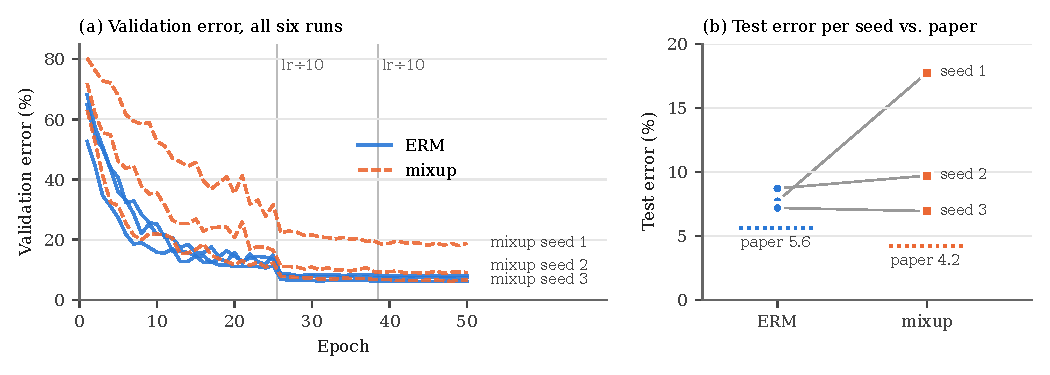
\includegraphics[width=\textwidth]{generated/results.pdf}
\caption{(a) Validation error per epoch for all six runs; vertical lines mark the learning-rate
drops. (b) Test error of each selected checkpoint, with lines joining the two runs of a seed; dotted
lines are the paper's values. Seed~1 mixup is the outlier in both panels.}
\label{fig:results}
\end{figure*}

\section{What did not reproduce}
\subsection{The direction of the effect}
The paper reports a 1.4-point gain from mixup. I measured a mean change of $\DiffMean$\pp{}, with
mixup winning \MixWins{} of 3 pairs. The test gaps follow the validation gaps closely (seed~1:
validation \MixValOne\% vs \ErmValOne\%, test \MixTestOne\% vs \ErmTestOne\%), so checkpoint
selection transferred to the test set and the result is not a test-set accident.

\subsection{Consistency across seeds}
The mean hides two different outcomes. On seeds 2 and 3 the methods are within about a point
(differences of $\DiffTwo$ and $\DiffThree$\pp), and seed~3 favours mixup. Seed~1 is ten points apart.
The standard deviation across seeds is \MixSD\pp{} for mixup and \ErmSD\pp{} for ERM: at this budget
mixup's outcome depends on the seed far more than ERM's. The paper reports a single number per
method without the number of runs or their spread, so it is not possible to say whether this
variance is new or simply unreported.

With three seeds, a mean difference of $\DiffMean$\pp{} against a paired SD of \DiffSD\pp{} cannot
be separated from seed noise. I therefore make no significance claim either way. The honest summary
is that mixup with $\alpha=1$ did not deliver a reliable improvement at 50 epochs.

\section{What I tried, and why mixup fell short}
After the first pair of runs showed a validation gap of almost eleven points, and before the test set was
opened, I ran three checks on the seed~1 models using only training and validation data.

\subsection{Is it a bug?}
The paper notes that mixup becomes ERM as $\alpha\to0$. I trained a 5-epoch control with
$\alpha=0.001$, which still exercises the sampling, permutation, label pairing and mixed loss, but
almost always draws $\lambda$ near 0 or 1. Table~\ref{tab:check} shows that it tracks ERM, while
$\alpha=1$ does not. The control is not bit-identical to ERM, as expected, because reordering a
batch changes floating-point summation order. A bug in the mixup path would not leave $\alpha\to0$
behaving like ERM, so I rule it out as the main cause.

\begin{table}[t]
\caption{Code-path check: validation error (\%) in the first five epochs}
\label{tab:check}
\centering
\small
\begin{tabular}{@{}lrrrrr@{}}
\toprule
Seed 1, epoch & 1 & 2 & 3 & 4 & 5\\
\midrule
ERM & 64.82 & 54.60 & 50.14 & 43.52 & 35.94\\
mixup, $\alpha=0.001$ & 64.02 & 53.42 & 43.80 & 41.58 & 31.16\\
mixup, $\alpha=1$ & 80.30 & 76.28 & 72.76 & 72.08 & 67.96\\
\bottomrule
\end{tabular}

\end{table}

\subsection{Underfitting or overfitting?}
I measured the error of the selected models on 5,000 clean (unmixed, unaugmented) training images
(Table~\ref{tab:diagnostic}). ERM fits them almost perfectly (\ErmCleanTrain\%). mixup misclassifies
\MixCleanTrain\%, close to its validation error. The mixup model is not failing to generalize; it
has not finished learning the training set. This is a number the paper does not report, and it is
the clearest explanation of the gap.

\subsection{Batch normalization statistics}
A network trained on mixed images collects batch-normalization~\cite{ioffe2015batchnorm} running
statistics from mixed inputs, but is evaluated on clean ones. Re-estimating those statistics on
unmixed training batches improved mixup's validation error by only \MixBNGain\pp{} (ERM:
\ErmBNGain\pp). The mismatch is real but small, and not the main cause.

\begin{table}[t]
\caption{Seed 1 diagnostic: validation and clean-training error (\%)}
\label{tab:diagnostic}
\centering
\small
\begin{tabular}{@{}lrrrr@{}}
\toprule
& \multicolumn{2}{c}{As trained} & \multicolumn{2}{c}{BN re-estimated}\\
\cmidrule(lr){2-3}\cmidrule(lr){4-5}
Seed 1 & Val. & Clean train & Val. & Clean train\\
\midrule
ERM & 7.20 & 0.46 & 7.14 & 0.44\\
mixup & 17.98 & 15.72 & 16.94 & 14.58\\
\bottomrule
\end{tabular}

\end{table}

\subsection{Why seed 1}
Seed~1's mixup run started badly. Its first-epoch training objective was \MixOneObjEpochOne, above
$\ln 10\approx2.30$, the loss of a uniform guess, and its validation error after one epoch was
\MixOneValEpochOne\% against \MixTwoValEpochOne\% for seed~2. It stayed behind for the whole run
(Fig.~\ref{fig:results}a). This run was also interrupted after epoch 5 and resumed; its history is
continuous across the resume, and a later resume of seed~2 on a new Colab runtime reproduced the
interrupted epoch's validation error exactly, so the resume is not the cause.

\subsection{Reading this against the paper}
The paper itself says, in its ImageNet section, that large $\alpha$ leads to underfitting and that
longer training runs benefit most from mixup. Its CIFAR-10 result combines the largest $\alpha$ it
uses with 200 epochs. Cutting the schedule to 50 epochs removes the regime in which the paper says
mixup pays off, and the underfitting I measured is consistent with that. My results do not show that
mixup fails at full scale; they show that the claimed gain is not robust to a fourfold shorter
schedule, which the paper does not mention.

\section{Gaps in the paper}
\label{sec:gaps}
Reproducing the claim exposed details the paper leaves open. (i)~It does not state how many runs
the 5.6\% and 4.2\% come from, or their spread. (ii)~It does not say whether these are final-epoch
errors or the best test error during training. The authors' script evaluates the test set every
epoch and saves the checkpoint with the best test accuracy, and the paper's corrupted-label table
explicitly reports the best test error during training. If Fig.~3(a) uses the same rule, the model
was selected on the test set, which biases both numbers downward. (iii)~The learning-rate schedule
and $\alpha$ are given for 200 epochs only, with no guidance for shorter budgets. I had to choose
the compressed milestones (25 and 38) myself.

\section{Engineering notes}
A typical epoch took \EpochSeconds~s on a T4, so the six runs need about \GpuHours~GPU-hours, with peak
GPU memory near \PeakGpuMB~MB; the paper reports neither. Checkpoints were saved every five epochs
to Google Drive, and the connection to Colab dropped three times. After one drop, epoch times
doubled for 25 epochs, which fits a second copy of the resumed run sharing the GPU with the
original. Because training is deterministic on the same GPU, both copies would compute identical
values, and a pre-freeze check
confirmed that every checkpoint loaded, covered all 50 epochs and matched its history. Every
interruption, check and decision is in the repository's experiment log, including the decision,
recorded before the test set was opened, to keep $\alpha$ and the schedule unchanged.

\section{Limitations and next step}
Three seeds are too few to estimate mixup's variance well, and the comparison holds only for this
protocol. The obvious next step is to repeat the paper's numbers at 200 epochs. The more useful one
is to vary the schedule length (for example 50, 100 and 200 epochs) at $\alpha=1$ and $\alpha=0.2$,
since the open question is how long mixup needs to train before it helps, and whether a smaller
$\alpha$ helps sooner. Either would be a new, separately labelled experiment; the frozen results
reported here would not change.

\section*{Reproducing this report}
From a clean checkout, in the conda environment described in the README,
\begin{center}
\footnotesize\verb|python scripts/reproduce.py --from-results results|
\end{center}
checks the committed results against the freeze manifest and the code, and regenerates every
number, table and figure in this paper. Running it with \verb|--data| and \verb|--output| instead
reruns all training and evaluation on a GPU first.

\section*{Use of AI tools}
Claude Code (Anthropic) helped write and debug code and draft this report. I ran the experiments,
checked every number against the repository, and am responsible for the content.

\bibliographystyle{IEEEtran}
\bibliography{references}

\end{document}
